\documentclass[tikz]{standalone}


\usetikzlibrary{shapes, shapes.geometric, shapes.misc, shapes.arrows}
\usetikzlibrary{angles, math, calc, matrix}
\usetikzlibrary{circuits.ee.IEC}

\begin{document}
    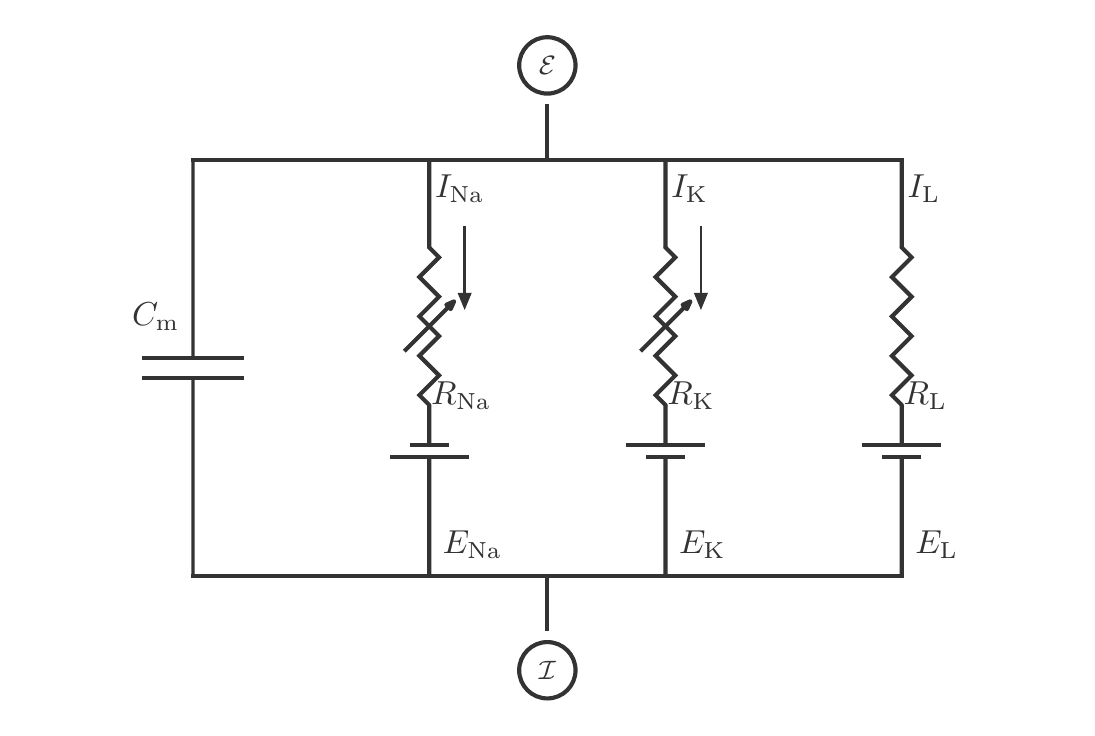
\begin{tikzpicture}[
    %x=1cm, y=1cm, 
    %z={(0cm,1cm)},
    scale = 1.2,
    transform shape,
    line width = 1.5pt, 
    black!80,
    circuit ee IEC,
    every info/.style={font=\footnotesize},
        small circuit symbols,
            set resistor graphic=var resistor IEC graphic,
            set diode graphic=var diode IEC graphic,
            set make contact graphic= var make contact IEC graphic
    ]

    % Determines the boundries
    \path[use as bounding box] (-5.5,-3.6) rectangle (5.5,3.6);

    \def\r{0.5}             % radius of heads
    \def\s{0.5}             % scale
    \def\l{2}               % length
    \def\w{0.75}            % width
    \def\wl{1}              % width of the lipids
    \def\wc{1.30}           % width of the capacitor
    \def\j{2cm}             % not too sure
    \def\chanGap{3cm}
    \def\exShift{3}
    \def\steps{4}

    % Ratio for each ion
    \def\Nar{1/3}
    \def\Kr{2/3}
    \def\Lr{10/10}
    \def\Nas{Na}
    %\def\Kr{3/12}
    %\def\Nar{7/12}
    %\def\Nar{1/(2*\r*\s)}
    \def\Clr{11/12}

    % Definining the coordinates of the box corners
    \def\boxRise{2.2}
    \def\boxRun{3.75}
    
    \coordinate (O)  at (0,0);
    \coordinate (TR) at ( \boxRun, \boxRise);
    \coordinate (TL) at (-\boxRun, \boxRise);
    \coordinate (BL) at (-\boxRun,-\boxRise);
    \coordinate (BR) at ( \boxRun,-\boxRise);

    % Define centers of the walls of the circuit
    \coordinate (CC) at ($(TL)!1/2!(BL)$);
    \coordinate (LC) at ($(TR)!1/2!(BR)$);
    
    % Define centers of the floor and ceiling of the circuit
    \coordinate (EM) at ($(TL)!1/2!(TR)$);
    \coordinate (IM) at ($(BL)!1/2!(BR)$);

    
    % Underlines Circuit
    \begin{scope}[white, line width = 5pt]
              
    % Leakage
    \draw ($(TL)!\Lr!(TR)$) to [resistor={pos = 0.40}, 
        battery={pos = 0.70, minimum height=0.75cm, minimum width=0.15cm, line cap = rect}]  %node [pos = 0.5, anchor = north west, xshift = -3.5]{$R_\mathrm{L}$} 
            ($(BL)!\Lr!(BR)$);

          
    % Outlines circuit
    \draw[line cap = rect] (TL) -- ($(TL)!\Lr!(TR)$) 
                           (BL) -- ($(BL)!\Lr!(BR)$);
    \end{scope}
        
    \begin{scope}[line width = 1.5pt] % Draws the visible circuit
        % Marks the extternal Nodes
        \path ( 90: \boxRise + 1)  node (E) [circle, minimum width = 0.77cm, fill = white]{};
        \path (-90: \boxRise + 1) node  (I) [circle, minimum width = 0.77cm, fill = white]{};

    
        % Node to Cicuit
        \draw[white, line width = 5pt] 
              (E) to (EM)
              (I) to (IM);

              
        % Node to Cicuit
        \draw (E) to (EM)
              (I) to (IM);

         % Node to Cicuit  
        \node at (I) [circle,draw, fill = white] {\footnotesize $\mathcal{I}$};
        \node at (E) [circle,draw, fill = white] {\footnotesize $\mathcal{E}$};
        
        % Outlines circuit
        \draw[line cap = rect] (TL) -- ($(TL)!\Lr!(TR)$) 
                               (BL) -- ($(BL)!\Lr!(BR)$);



        % Internal labeling and circutry
        \begin{scope}[align=left]
        \foreach \F/\I/\R/\A in 
            {\Nar/Na/0/adjustable', \Kr/K/180/adjustable', \Lr/L/180/}{
            % Making the main circuit paths
            \draw ($(BL)!\F!(BR)$) to 
            [battery={pos = 0.30, minimum height=1cm, minimum width=0.15cm, rotate = \R, line width = 1.2pt}, 
             resistor={\A, pos = 0.60, minimum height=0.25cm, minimum width = 2cm}] 
                node[pos = 0.5, anchor = north west, xshift = -3.5]
                {$R_\mathrm{\I}$} ($(TL)!\F!(TR)$);
    
            % Making external markings
            \path ($(TL)!\F!(TR)$) -- ($(BL)!\F!(BR)$) node (I\I) 
                [pos = 0.069, anchor = west, inner sep = 1pt]  
                {$I_{\mathrm{\I}}$};
            
            \path ($(TL)!\F!(TR)$) -- ($(BL)!\F!(BR)$) node (E\I) 
                [pos = 0.925, anchor = west]  
                {$E_{\mathrm{\I}}$};
    
            \foreach \o in {-,+}{
                \path ($(TL)!\F!(TR)$) -- ($(BL)!\F!(BR)$) 
                    node (S\I\o) [pos = 0.70, anchor = east, inner sep=0pt, xshift = -0.35cm, yshift = \o 0.28 cm]  {};
            }
        }
    
        % Arrows
        \foreach \i in {\Kr, \Nar}{
            \draw[line width = 1pt] ($(TL)!\i+0.05!(TR)$)++(0,-0.70cm) -- ++(0,-0.75cm) 
            node[isosceles triangle, scale = 0.25, draw, fill, rotate = 270] 
            {};
        }

        % Arrowing each side
        \path ($(BL)!\Nar/2!(BR)$) -- +(0, 0.25) coordinate (BE)
              ($(TL)!\Nar/2!(TR)$) -- +(0,-0.25) coordinate (TE);
        \end{scope}
        
        % Capacitance shit
        \draw[line cap = rect, line width = 1.2pt]  (BL) to 
            [capacitor={minimum height= \wc cm, minimum width = 0.25 cm}] (TL);
        \path (BL) -- (TL) node[midway, anchor = south east, yshift = 0.25cm] {$C_\mathrm{m}$};

        \path (CC)++( 90:\l * \s +  \r * \s  + \exShift * \s  cm) -- +(0:0.5*\wc) coordinate (PR) -- +(180:0.5*\wc) coordinate (PL);
        \path (CC)++(-90:\l * \s +  \r * \s  + \exShift * \s  cm) -- +(0:0.5*\wc) coordinate (NR) -- +(180:0.5*\wc) coordinate (NL);

    \end{scope}
    \end{tikzpicture}
\end{document}